\RequirePackage{luatex85}
\documentclass[tikz, border=10pt]{standalone}

\usepackage[compat=1.1.0]{tikz-feynman}

\begin{document}
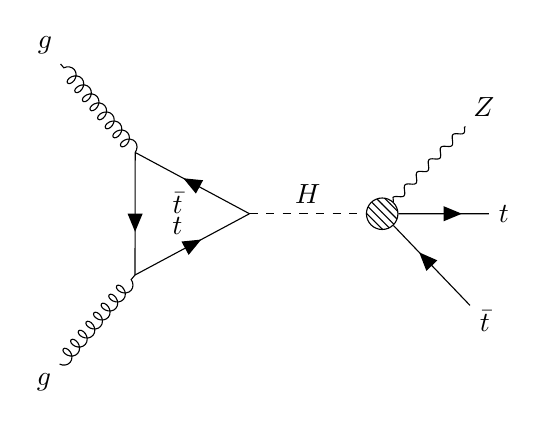
\begin{tikzpicture}
  \begin{feynman}
    \diagram [horizontal=c to d] {
      i1 [particle=\(g\)] -- [gluon] a -- [anti fermion] b -- [gluon] i2 [particle=\(g\)],
      a -- [fermion, edge label=\(t\)] c -- [fermion, edge label=\(\bar{t}\)] b,
      c -- [scalar, edge label=\(H\)] d [blob, minimum size=0.4cm],
      f1 [particle=\(Z\)] -- [boson] d,
      f2 [particle=\(t\)] -- [anti fermion] d -- [anti fermion] f3 [particle=\(\bar{t}\)],
      f1 -- [opacity=0] f2 -- [opacity=0] f3,
    };
  \end{feynman}
\end{tikzpicture}
\end{document}
